\documentclass[a4paper,12pt]{article}
\usepackage{amsmath,amsfonts,amsthm,amssymb, mathtools,steinmetz, gensymb, siunitx}	% LOADS USEFUL MATH STUFF
\usepackage{xcolor,graphicx}
\usepackage[a4paper]{geometry} 				% ADJUSTS PAGE
\usepackage{setspace}
\usepackage{physics}
\usepackage{caption}
\usepackage{tikz}
\usepackage{pgf,tikz,pgfplots}
\usepackage{mathrsfs}
\usepackage{amsbsy}
\usepackage{fancyhdr}
\usepackage{float}
\usepackage{array}
\usepackage{booktabs}
\usepackage{newpxtext}
\usepackage{unicode-math}
\usepackage{braket}
\setmathfont{Libertinus Math}

\usetikzlibrary{decorations.pathreplacing,decorations.markings}
\usepgfplotslibrary{fillbetween}

\newgeometry{left=1cm,top = 2.5cm, bottom = 1.75cm, right = 1cm}

\newcommand{\defeq}{:=}
\newcommand\block[1]{\hspace*{#1}}
\newcommand{\rpm}{\sbox0{$1$}\sbox2{$\scriptstyle\pm$}
	  \raise\dimexpr(\ht0-\ht2)/2\relax\box2 }
\newcommand{\af}{\pmb{\hat a_1}}
\newcommand{\as}{\pmb{\hat a_2}}
\newcommand{\at}{\pmb{\hat a_3}}
\newcommand\uv[1]{\pmb{\hat {#1}}}
\newcommand\vect[1]{\pmb{{#1}}}
\newcommand\rbm[1]{\left(\begin{matrix} {#1} \end{matrix}\right)}
\newcommand\dprod{\pmb{\cdot}}
	  
\pgfplotsset{compat=newest}
\newlength{\QNo}
\settowidth{\QNo}{2.}

\newlength{\QLetter}
\settowidth{\QLetter}{(a)}

\pagestyle{fancy}
\rhead{Quantum mechanics Problem Set}
\lhead{J. L. Gouws}


\begin{document}
\fontencoding{T1}
\fontfamily{ppl}\selectfont
{\Large \textbf{Quantum mechanics Assignment 1}} \hfill {\Large \textbf{J L Gouws}}\\
\block{1.0cm} {\large \textbf{\today}} \hfill {\large \textbf{26634554}}\\
\thispagestyle{empty}
\fontencoding{T1}

1.
\begin{minipage}[t]{0.9\textwidth}
  \begin{align*}
    \left(\bra{\psi} + \alpha^* \bra{\phi}\right)\left(\alpha \ket{\phi} + \ket{\psi}\right) &= \bra{\psi}\left(\alpha \ket{\phi} + \ket{\psi}\right) + \alpha^* \bra{\phi}\left(\alpha \ket{\phi} + \ket{\psi}\right)\\
                                                                                             &= \alpha \braket{\psi|\phi} + \braket{\psi|\psi} + |\alpha|^2 \braket{\phi | \phi}+ \alpha^*\braket{\phi|\psi}\\
                                                                                             & \geq 0\\
  \end{align*}
  The above statement holds for all $\alpha$, and in particular $\alpha = i\frac{\braket{\psi|\phi}}{\braket{\phi | \phi}}$.
  If we substitute this choice of $\alpha$ into the inequality above, we get:
  \begin{align*}
    \Rightarrow & i \frac{|\braket{\psi|\phi}|^2}{\braket{\phi|\phi}} + \braket{\psi|\psi} - |\braket{\psi|\phi}|^2\frac{\braket{\phi | \phi}}{|\braket{\phi | \phi}|^2} - i \frac{|\braket{\phi|\psi}|^2}{\braket{\phi|\phi}} \geq 0\\
    \Rightarrow & \braket{\psi|\psi} - \frac{|\braket{\psi|\phi}|^2}{\braket{\phi | \phi}} \geq 0\\
    \Rightarrow & \braket{\psi|\psi} \braket{\phi | \phi} \geq |\braket{\psi|\phi}|^2\\
  \end{align*}
  Which is the required result. 
\end{minipage}

\iffalse
\begin{figure}
  \centering
  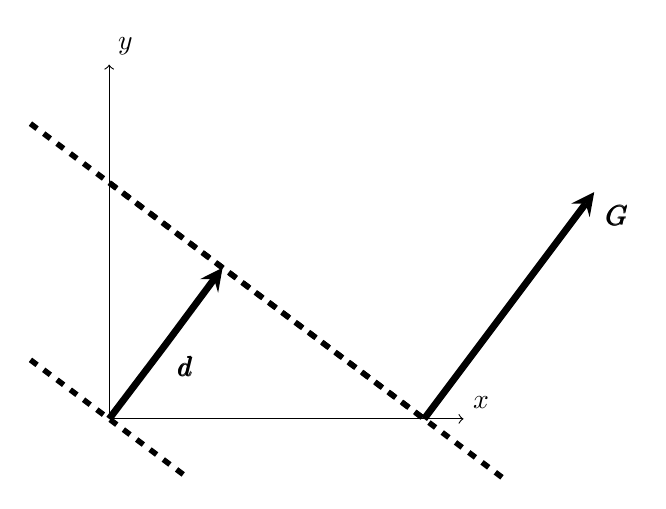
\begin{tikzpicture}
    \draw[->] (0, 0) -- (4.5, 0) node[anchor = south west] {$x$};
    \draw[->] (0, 0) -- (0, 4.5) node[anchor = south west] {$y$};
    \draw[dashed, line width = 2] (-1, 3.75) -- (5, -0.75);
    \draw[dashed, line width = 2] (-1, .75) -- (1, -0.75);
    \draw[dashed, line width = 2] (0, 3) -- (4, 0);
    \draw[->, line width = 2.5, >=stealth] (0, 0) --  (0.72, 0.95) node[anchor = north west] {$\pmb{d}$}-- (1.44, 1.92);
    \draw[->, line width = 2.5, >=stealth] (4, 0) -- (6.16, 2.88) node[anchor = north west] {$\pmb{G}$};
  \end{tikzpicture}
  \caption{The interplanar separation.}
  \label{fig:planeSep}
\end{figure}

\begin{figure}
  \centering
  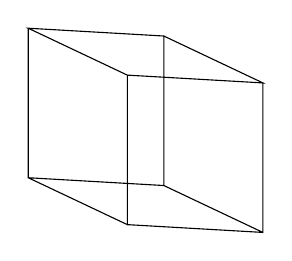
\begin{tikzpicture}
    \begin{axis}[
      axis x line=none,
      axis y line=none,
      axis z line=none,
      axis equal image,
%      view = {20}{30}
    ]
    \addplot3 [mark=none] coordinates 
    {
      (0, -1, 2)
      (3, 0, 2)
      (0, 1, 2)
      (-3, 0, 2)
      (0, -1, 2)
      (0, -1, -2)
      (3, 0, -2)
      (3, 0, 2)
      (3, 0, -2)
      (0, 1, -2)
      (0, 1, 2)
      (0, 1, -2)
      (-3, 0, -2)
      (-3, 0, 2)
      (-3, 0, -2)
      (0, -1, -2)
      (0, -1, 2)
      (0, -1, -2)
    };
    \end{axis}
  \end{tikzpicture}
  \caption{The first Brillouin zone of a hexagonal lattice}
  \label{fig:firsBrillouin}
\end{figure}
\fi

2.
\begin{minipage}[t]{0.9\textwidth}
  a).
  \begin{minipage}[t]{\textwidth}
    Let $\left(\begin{matrix} a & b \\ c & d\end{matrix}\right)$ be a general matrix over $\mathbb{C}$.\\
    Then we need to find $\alpha, \beta, \gamma, \delta \in \mathbb{C}$, such that:
    \begin{equation*}
      \left(\begin{matrix} a & b \\ c & d\end{matrix}\right) = \alpha \left(\begin{matrix}1 & 0 \\ 0 & 1\end{matrix}\right)
        + \beta \left(\begin{matrix}0 & 1 \\ 1 & 0\end{matrix}\right) + \gamma \left(\begin{matrix}0 & -i \\ i & 0\end{matrix}\right) + \delta\left(\begin{matrix}1 & 0 \\ 0 & -1\end{matrix}\right)
    \end{equation*}
    For this we have:
    \begin{align*}
      a &= \alpha + \delta\\
      b &= \beta + -i\gamma\\
      c &= \beta  + i\gamma\\
      d &= \alpha - \delta
    \end{align*}
    This system of equations is partially decoupled, and so is easily solved.
    \begin{align*}
      \alpha  &= \frac{a + d}{2}\\
      \beta &= \frac{b + c}{2}\\
      \gamma &= i\frac{b - c}{2}\\
      \delta &= \frac{a - d}{2} 
    \end{align*}
    Since $a, b, c, d$ are in $\mathbb{C}$ and $\mathbb{C}$ is a field, $\alpha, \beta, \gamma, \delta$ are definitely in $\mathbb{C}$ as required.
  \end{minipage}

  b).
  \begin{minipage}[t]{\textwidth}
    $\trace\left({A^\dagger B}\right)$ is an inner product:
    First, $\left(A, B\right) = \trace\left(A^\dagger B\right)$, is indeed a map $\mathbb{C}^{2\times 2}\times \mathbb{C}^{2\times 2} \to \mathbb{C}$.\\
    Let:
    \begin{equation*}
      A = \rbm{a & b \\ c & d}
    \end{equation*}
  \end{minipage}

\end{minipage}
\end{document}
